
\section{Detekcia objektu v~obraze}
\label{sec:detekcia}

V~prvom rade je potrebné povedať že detekcia objektu a klasifikácia v~obraze je veľmi dobre známy problém v~oblasti spracovania obrazu.
V~dnešnej dobe už niektoré modely prebehli svojou presnosťou a výkonom aj človeka \cite{prop:NNvsHuman}.

Rozoberaním problému lokalizácie a správnej klasifikácie objektu v~obraze, skončíme s~potrebou
    detekcie a klasifikácie niekoľkých objektov súčasne v~jednej scéne.
Detekcia objektu v~obraze je problém pozostavajúci z~hľadania a klasifikovania variabilného počtu a rôznych typov objektov v~obraze.
Dôležitým rozdielom je ``variabilná'' časť. V~porovnaní s~klasifikáciou je výstup detekcie objektov rôznorodý svojou dĺžkou, keďže
    počet objektov v~obraze sa môže meniť z~obrázka na obrázok \cite{odkaz:ObjectDetectionOverview}.

\subsection{Prehľad existujúcich riešení}

\subsubsection{Klasický prístup}
Aj keď v~priebehu rokov bolo množstvo rôznych typov riešení, pre túto prácu je vhodné spomenúť 2 hlavné prístupy.

Prvý z~nich je Viola-Jones spôsob, ktorý navrhol v~roku 2001 Paul Viola a Michael Jones v~práci \cite{prop:Viola2001RobustRF}.
Tento prístup je rýchly a relatívne jednoduchý, až natoľko, že sa tento algoritmus implementuje v~kamerách s~bodovým snímačom, ktorý umožňuje
    detekciu tvári v~reálnom čase s~malým množstvom potrebného výkonu.
V~jednoduchosti, algoritmus generuje rôzne, môže až tisíce, jednoduché binárne klasifikátory pomocou tzv. Haar funkcií.
Tieto klasifikátory sú kaskádovito zoradené a vyhodnocované v~poradí podľa ich zložitosti, s~využitím viacnásobného posuvného okna [eng. multi-scale sliding window].
V~prípade negatívnej klasifikácie v~ktorejkoľvek úrovni vyhodnocovania, je tento proces ukončený a pokračuje sa klasifikáciou nad ďalším podoknom (angl. \textit{subwindow}) \cite{prop:Viola2001RobustRF}.

Druhý spôsob je klasifikácia pomocou histogramu orientovaných prechodov (angl. \textit{histogram of oriented gradients}) a Support Vector Machine, ktorý bude podrobne
    rozobratý v~kap. \ref{sec:klasifikacia}. Tento prístup takisto používa viacnásobné posuvné okno, avšak aj keď je lepší ako Viola-Jones, je oveľa pomalší \cite{odkaz:ObjectDetectionOverview}.

\subsubsection{Prístup pomocou hlbokých neurónových sietí}
S~príchodom neurónových sietí prišla aj veľká zmena v~oblasti spracovania obrazu, preto je vhodné spomenúť niekoľko spôsob
    detekcie objektov ktoré stavajú na neurónových sieťach.

\textbf{R-CNN} je jeden z~prvých riešení \cite{prop:rcnn}, v~ktorom navrhovali 3 stupňový prístup:
\begin{enumerate}
	\item[$\bullet$] extrahovať možné objekty pomocou metódy regionálnych návrhov (angl. \textit{region proposal}),
    \item[$\bullet$] extrahovať príznaky z~každého regiónu pomocou konvolučných neurónových sietí,
    \item[$\bullet$] klasifikovať každý región pomocou Support Vector Machine.
\end{enumerate}

\textbf{Fast R-CNN} je označenie pre prístup, ktorý vylepšil predchádzajúci R-CNN, základom je, že stavia už iba na využítí konvolučných neurónových sietí.
V~práci použili dva prístupy k~detekcii objektu, sliding window a region proposal.
Výsledky ukázali, že prístup pomocou regionálnych návrhov (angl. \textit{region proposals}) bol rýchlejší a dosiahli rýchlosť spracovania až 2 snímkov za sekundu \cite{prop:fast-rcnn}.
\begin{figure}[H]
    \centering
    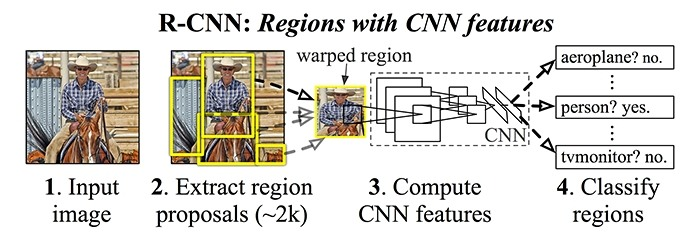
\includegraphics[width=0.8\textwidth]{rcnn}
    \qquad
    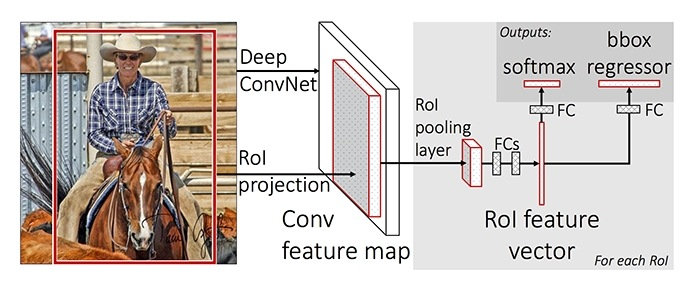
\includegraphics[width=0.6\textwidth]{fast-rcnn}
    \caption{Porovnanie architektúr R-CNN(hore) a Fast R-CNN(dole) \cite{odkaz:ObjectDetectionOverview}.}
    \label{pic:FastRCNN}
\end{figure}

\textbf{YOLO} (angl. \textit{You Only Look Once}), rieši problém detekcie objektu v~obraze ako regresívny problém.
Namiesto bežného postupu ako je najprv použitie techniky regionálnych návrhov a následne klasifikovanie týchto regiónov.
To vedie YOLO k~veľmi rýchlemu spracovaniu v~reálnom čase ale za cenu presnosti.
Týmto spôsobom YOLO dokáže dosiahnuť 63.4\% mAP, kde mAP je metrika pre určenie presnosti detekcie objektu v~obraze \cite{prop:metrics}, s~22 ms oneskorením \cite{prop:Redmon2016YouOL}.

\begin{comment}
    \subsubsection{Vyhľadávač na základe vizuálnej podobnosti obrázkov}
    Jednu z~možných aplikácií detekcie objektov v~obraze využíva Pinterest\footnote{\url{https://medium.com/@Pinterest_Engineering/introducing-automatic-object-detection-to-visual-search-e57c29191c30}}.
    Používaju detekciu objektov pre indexovanie rôznych častí obrázka.
    Týmto spôsobom si môže užívateľ pri hľadaní napr. špecifickej kabelky alebo topánok nájsť aj jej podobné.
    \begin{figure}[H]
        \centering
        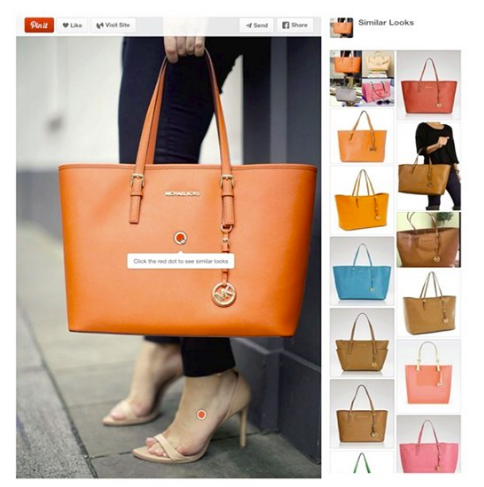
\includegraphics[width=0.5\textwidth]{purse}
        \caption{Prototyp automatického označovania a vyhľadávania objektov \cite{odkaz:ObjectDetectionOverview}}
        \label{pic:kNN}
    \end{figure}
\end{comment}

\subsection{Kĺzajúce okno}
\label{subsec:slidingwindow}
Kĺzajúce okno (angl. \textit{Sliding window}) je jedna z~metód pre detekciu objektov v~obraze.
Táto metóda je veľmi vyčerpávajúca pretože zakladá na veľkom počte kandidátnych okien, až $10^4$, vo vstupnom obrázku.
Metóda prechádza vstupný obrázok na všetkých lokáciách s~rôznou veľkosťou okna, následne sa na každom ``okne'' spúšťa klasifikátor.
Nevýhodou tohto prístupu je jeho časová náročnosť, preto sa tento spôsob nedá použiť pri spracovaní obrazu v~reálnom čase.
Ale na druhú stranu metóda poskytuje dobrú presnosť pri kvalitnom klasifikátore \cite{prop:AutomaticHandgunDetection}.

\subsection{Regionálne návrhy}
\label{subsec:regionproposal}
Metóda regionálnych návrhov (angl. \textit{region proposals}) na rozdiel od metódy kĺzajúceho okna, nepredpokladá za kandidátne okná všetky možnosti.
Tieto kandidátne okná sú vybrané pomocou metód návrhu detekcie (angl. \textit{detecion proposel methods}), konkrétne metódy
    a ich porovnanie je možné nájsť v~članku \textit{What makes for effective detection proposals?} \cite{prop:ProposalMethods}.
Prvý model na detekciu objektov, ktorý použil konvolučné neurónové siete s~touto metódou pre výber okien bol R-CNN \cite{prop:AutomaticHandgunDetection}.
